\chapter{Exigências Específicas}
	O sistema deve ser implementado contendo as funcionalidades referentes aos tópicos apresentados abaixo. Cada tópico será avaliado separadamente. Para o aluno obter nota máxima em cada tópico, ele precisa utilizar todas as estruturas listadas nos respectivos sub-tópicos. Também serão consideradas as boas práticas de programação em JavaScript, uso adequado de notações e conceitos aprendidos, organização do código e criatividade.

\section{Qualidade do código}
Estes itens foram retirado conforme combinado em sala de aula.
Style Guide
Strict mode
\subsection{Hint}
	Objetivo: mostrar a correção de apenas 5 problemas informados pelo lint ou hint.
	
Problema 1
\begin{figure}[!htb]
\setcounter{figure}{0}
\centering
\begin{minipage}{.5\textwidth}
  \centering
  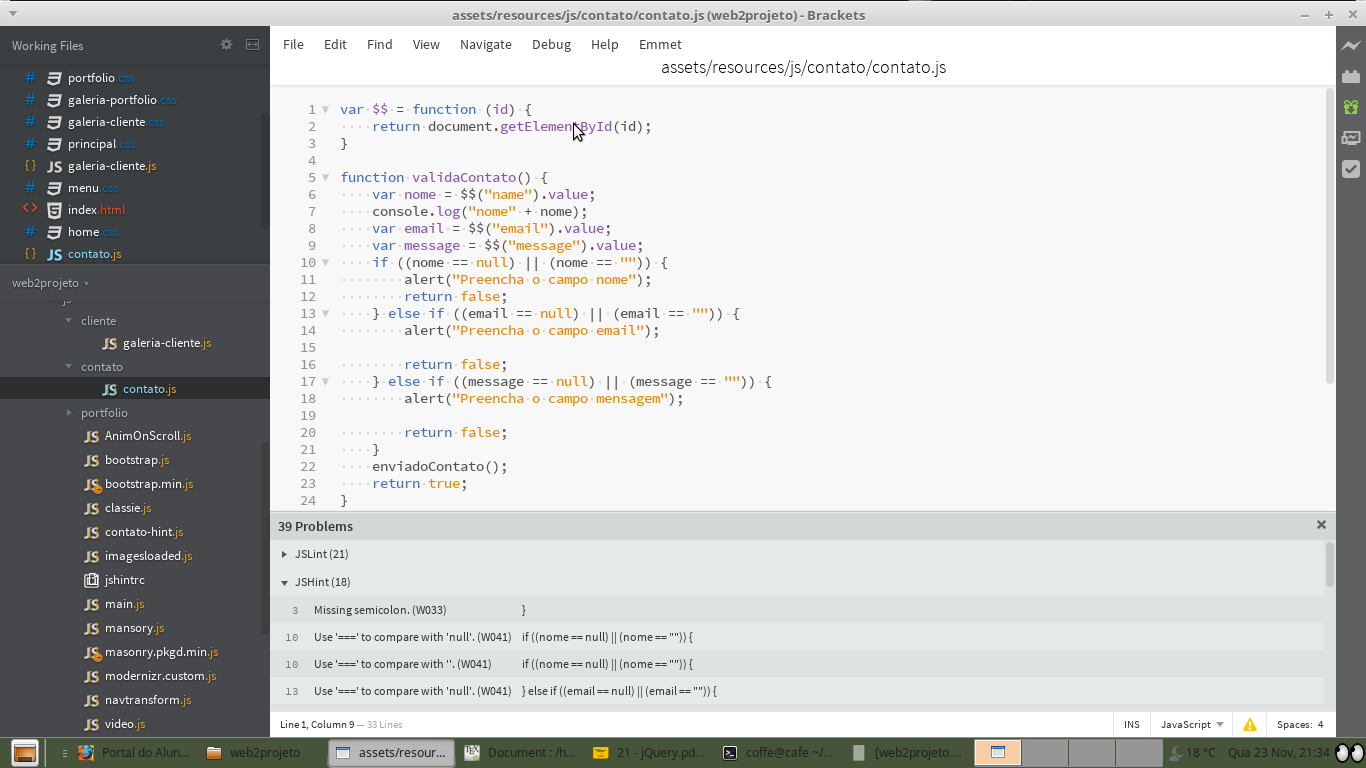
\includegraphics[width=.9\linewidth]{./img/hint1.png}
  \captionof{figure}{Problema 1}
\end{minipage}%
\begin{minipage}{.5\textwidth}
  \centering
  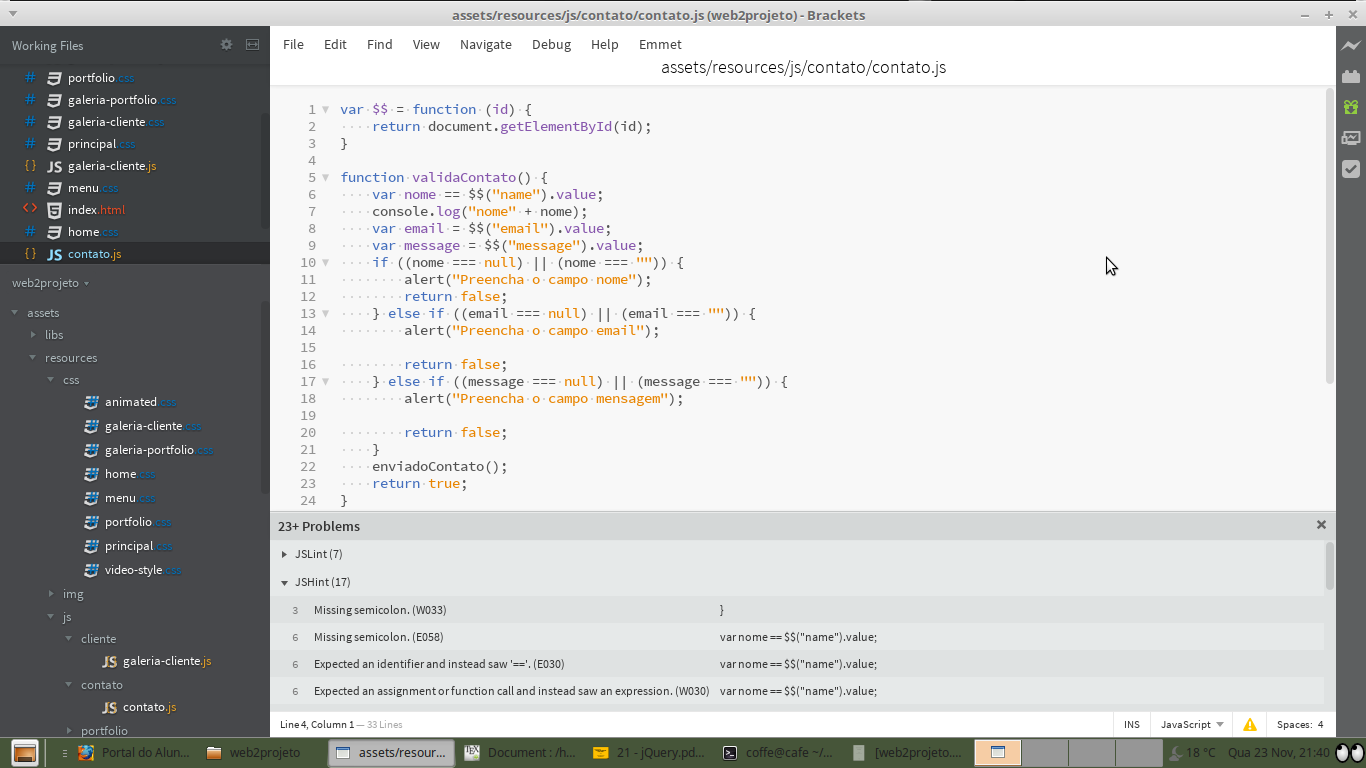
\includegraphics[width=.7\linewidth]{./img/hint1-arrumado.png}
  \captionof{figure}{Problema 1 - Correção}
\end{minipage}
\end{figure}	

Problema 2
\begin{figure}[!htb]
\setcounter{figure}{0}
\centering
\begin{minipage}{.5\textwidth}
  \centering
  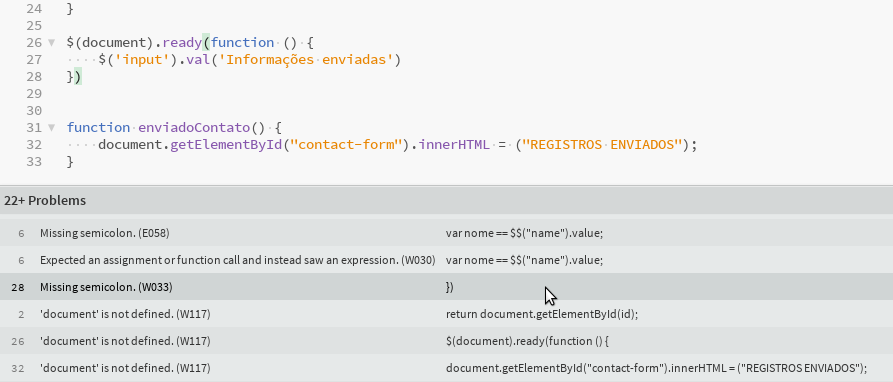
\includegraphics[width=.9\linewidth]{./img/hint2.png}
  \captionof{figure}{Problema 2}
\end{minipage}%
\begin{minipage}{.5\textwidth}
  \centering
  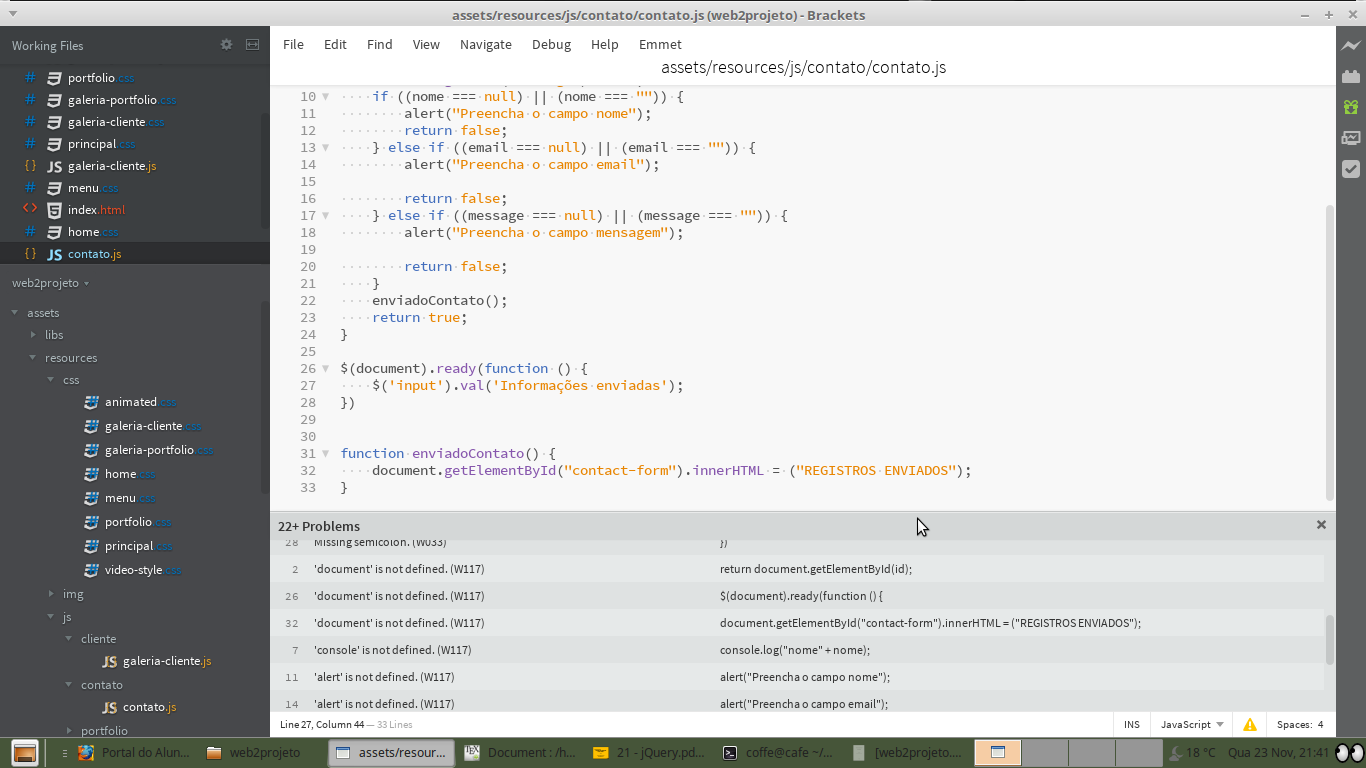
\includegraphics[width=.7\linewidth]{./img/hint2-arrumado.png}
  \captionof{figure}{Problema 2 - Correção}
\end{minipage}
\end{figure}	


Problema 3
\begin{figure}[!htb]
\setcounter{figure}{0}
\centering
\begin{minipage}{.5\textwidth}
  \centering
  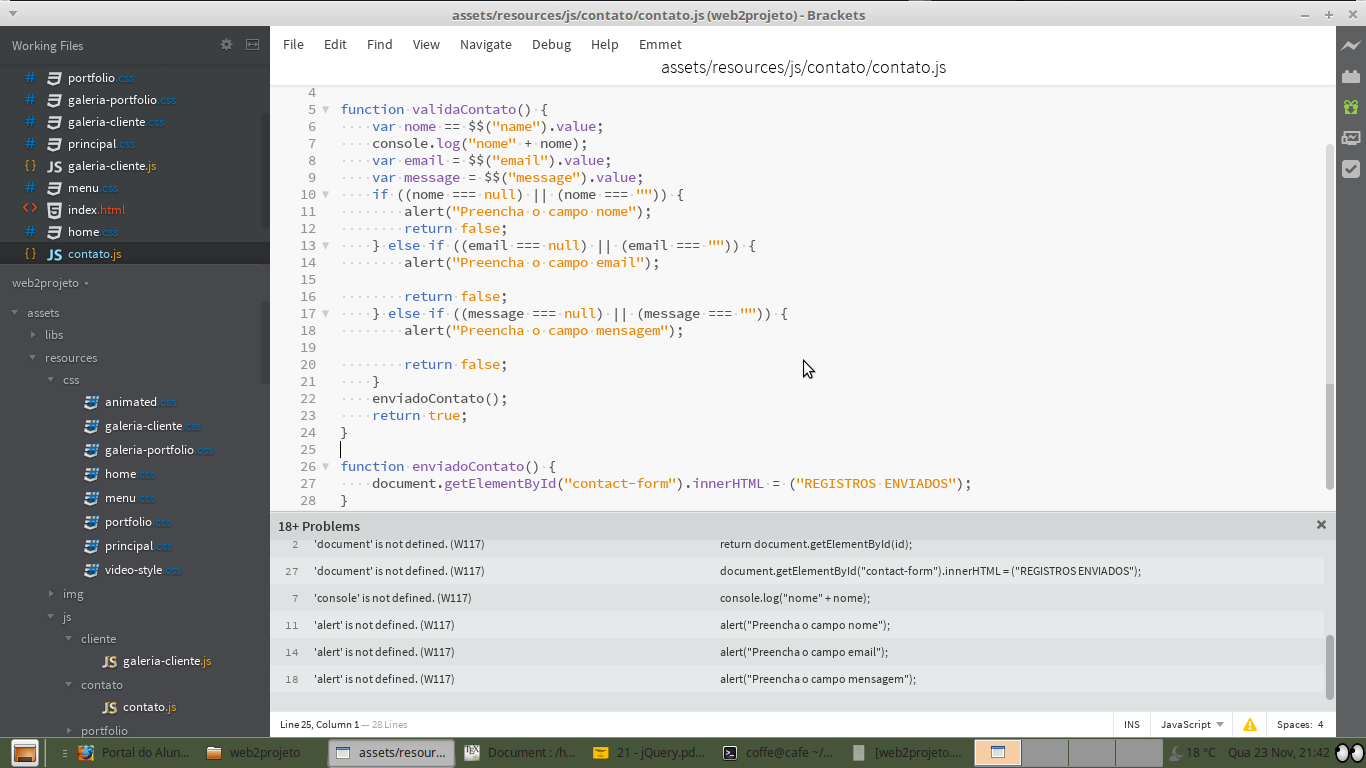
\includegraphics[width=.9\linewidth]{./img/hint3.png}
  \captionof{figure}{Problema 3}
\end{minipage}%
\begin{minipage}{.5\textwidth}
  \centering
  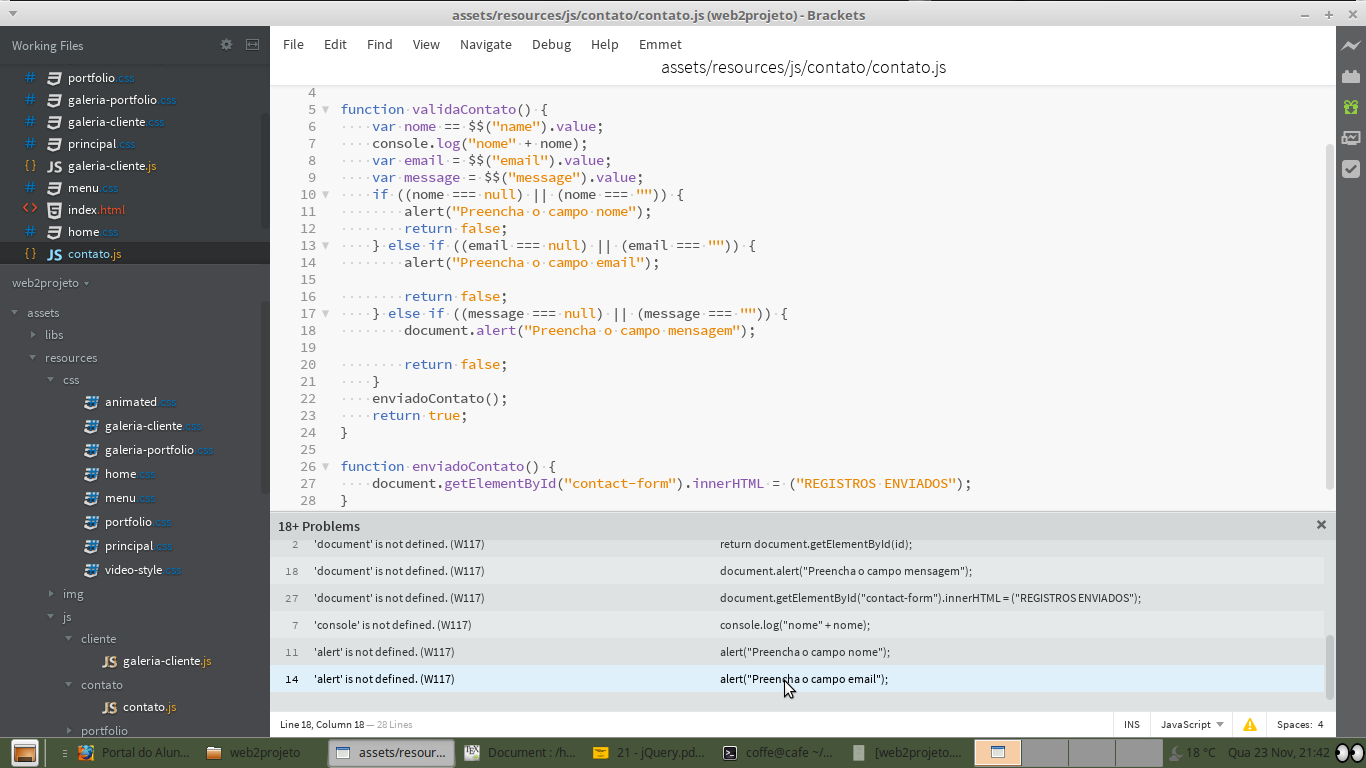
\includegraphics[width=.7\linewidth]{./img/hint3-arrumado.png}
  \captionof{figure}{Problema 3 - Correção}
\end{minipage}
\end{figure}

Problema 4
\begin{figure}[!htb]
\setcounter{figure}{0}
\centering
\begin{minipage}{.5\textwidth}
  \centering
  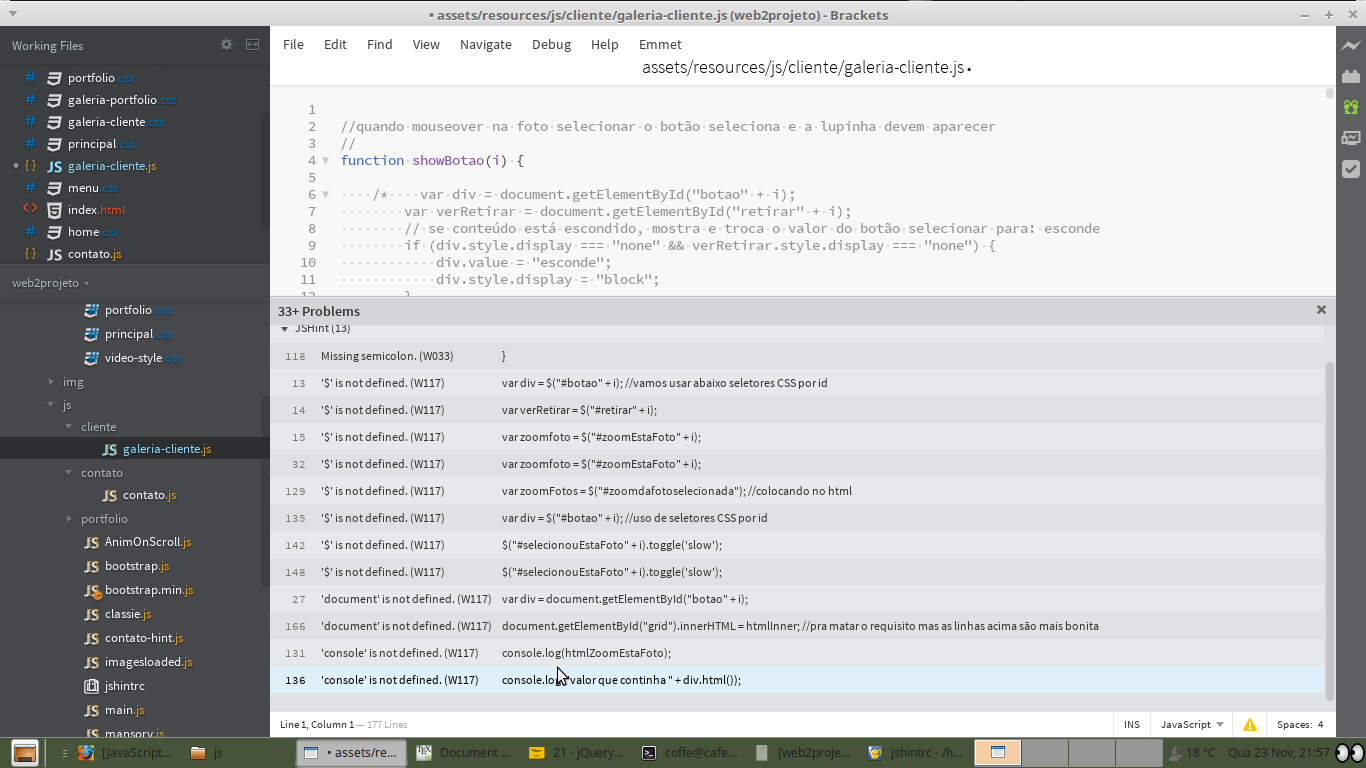
\includegraphics[width=.9\linewidth]{./img/hint4.png}
  \captionof{figure}{Problema 4}
\end{minipage}%
\begin{minipage}{.5\textwidth}
  \centering
  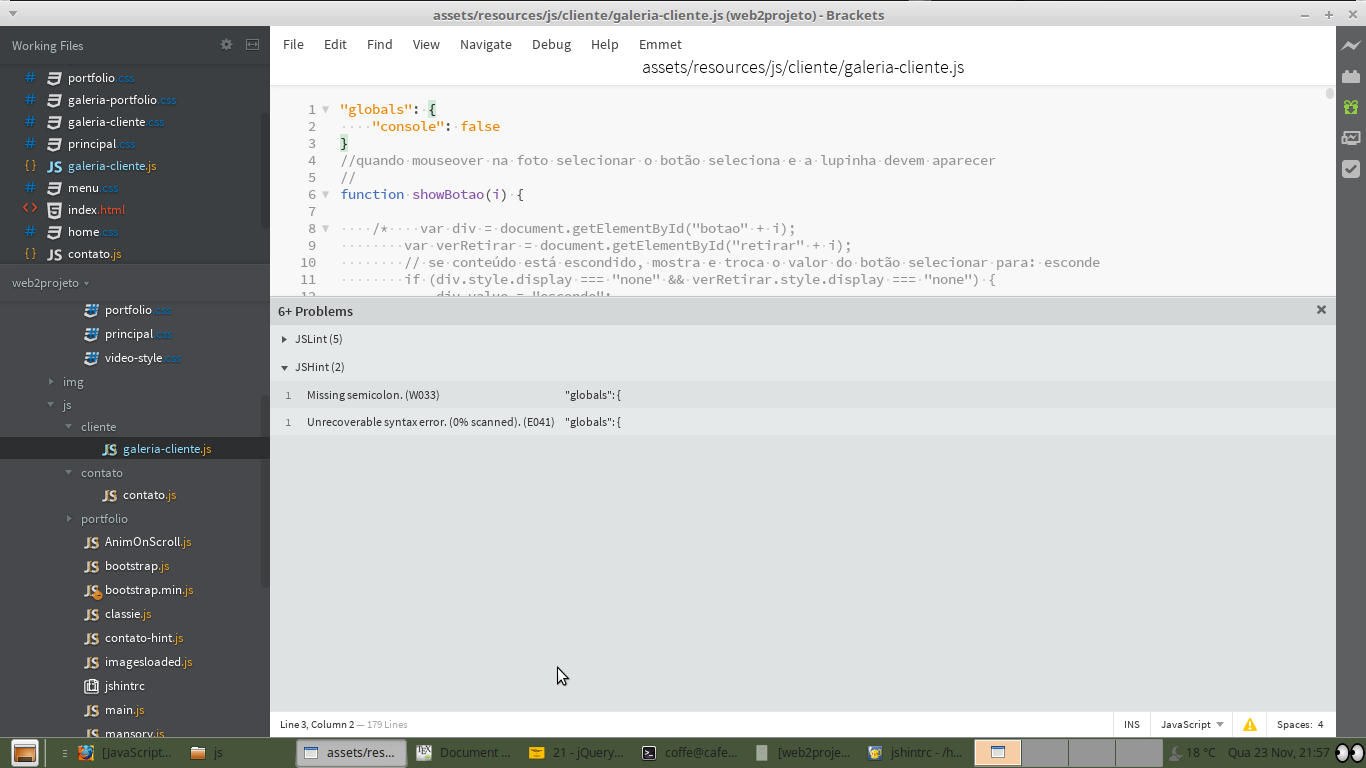
\includegraphics[width=.7\linewidth]{./img/hint4-arrumado.png}
  \captionof{figure}{Problema 4 - Correção}
\end{minipage}
\end{figure}	

\section{Caixas de Diálogo}

\subsection{prompt}

	Ver arquivo $galeria_cliente.js$
	
\begin{lstlisting}

function enviarFotosSelecionadas() {
    var confirma = confirm("Confirmar o envio das fotos?!");
    if (confirma == true) {
        var email = prompt("Por favor coloque um email para que possamos lhe comunicar sobre a entrega: ");
        //$(this).replaceWith($('<h5>' + this.innerHTML + '</h5>'));
        var fotosenviadas = { //comecamos armazenando email do cliente
            email: email
        };
        for (var i = 0; i < jsonClienteX.fotos.length; i++) {
            if (jsonClienteX.fotos[i].escolhido == true) {
                fotosenviadas[i] = jsonClienteX.fotos[i].arquivo; //armazenando todos os nomes dos arquivos
                console.log("enviando fotos" + i + "estava marcada no localstorage");
            }
        }
        var chaveParaAdmin = "FotosSalvasDe" + sessionStorage.getItem("logou");
        localStorage.setItem(chaveParaAdmin, JSON.stringify(fotosenviadas));
        localStorage.removeItem(sessionStorage.getItem("logou"));
        alert("Suas fotos foram enviadas Você será redirecionado para o inicio");
        deslogar();

    } else {
        return;
    }
}
\end{lstlisting}

\subsection{alert}

	No arquivo $JavaScript$ chamado $contato.js$ criamos uma função com nome $validaContato()$ conforme segue abaixo para melhor visualização:
	
\begin{lstlisting}
function validaContato() {
    var nome = $$("name").value;
    console.log("nome" + nome);
    var email = $$("email").value;
    var message = $$("message").value;
    if ((nome == null) || (nome == "")) {
        alert("Preencha o campo nome");
        return false;
    } else if ((email == null) || (email == "")) {
        alert("Preencha o campo email");
        return false;
    } else if ((message == null) || (message == "")) {
        alert("Preencha o campo mensagem");
        return false;
    }
    return true;
}
\end{lstlisting}
	Esta função está relacionada a validação dos campos do formulário. E dentro dela utilizamos $alert$ para enviar uma mensagem ao visitante da página.

\subsection{confirm}
	No arquivo $JavaScript$ chamado $galeria$\_$cliente.js$.
	Criamos uma função com nome $enviarFotosSelecionadas()$ conforme segue abaixo para melhor visualização:
	
\begin{lstlisting}
function enviarFotosSelecionadas() {
    var confirma = confirm("Confirmar o envio das fotos?!");
    if (confirma == true) {
        var email = prompt("Por favor coloque um email para que possamos lhe comunicar sobre a entrega: ");
        var fotosenviadas = { //comecamos armazenando email do cliente
            email: email
        };
        for (var i = 0; i < jsonClienteX.fotos.length; i++) {
            if (jsonClienteX.fotos[i].escolhido == true) {
                fotosenviadas[i] = jsonClienteX.fotos[i].arquivo; //armazenando todos os nomes dos arquivos
                console.log("enviando fotos" + i + "estava marcada no localstorage");
            }
        }
        var chaveParaAdmin = "FotosSalvasDe" + sessionStorage.getItem("logou"); //id do cliente sessionStorage.getItem("logou")
       
        localStorage.setItem(chaveParaAdmin, JSON.stringify(fotosenviadas));

        localStorage.removeItem(sessionStorage.getItem("logou"));

        alert("Suas fotos foram enviadas Você será redirecionado para o inicio");
        deslogar();

    } else {
        return;
    }
}
\end{lstlisting}
	Observe que na segunda linha da função temos o solicitado.

\section{Funções}
\subsection{Função anônima com argumento}
	No arquivo $JavaScript$ chamado $login.js$ criamos uma função anônima que receberá um argumento $i$ conforme segue abaixo para melhor visualização:
	
\begin{lstlisting}
var naoLogou = function (i) {
    var logou;
    if (i == 23) {
        sessionStorage.setItem("logou", "1267");
    }
}
\end{lstlisting}

\subsection{Função anônima sem argumento}

\subsection{Função anônima auto-executável}
	Ver no arquivo $contato.js$

\begin{lstlisting}
(function () { 
    tagDesnegrito();
});

\end{lstlisting}

\subsection{Função com nome}

	No arquivo $JavaScript$ chamado $contato.js$ criamos uma função com nome $validaContato()$ conforme segue abaixo para melhor visualização:
\begin{lstlisting}
function validaContato() {
    var nome = $$("name").value;
    console.log("nome" + nome);
    var email = $$("email").value;
    var message = $$("message").value;
    if ((nome == null) || (nome == "")) {
        alert("Preencha o campo nome");
        return false;
    } else if ((email == null) || (email == "")) {
        alert("Preencha o campo email");
        return false;
    } else if ((message == null) || (message == "")) {
        alert("Preencha o campo mensagem");
        return false;
    }
    return true;
}
\end{lstlisting}
	Esta função está relacionada a validação dos campos do formulário.

\subsection{Função aninhada/interna}

	Esta função está relacionada a construção de uma $grid$ de fotos do cliente, uma galeria de fotos. A função  $exibirFotosAoIniciar()$ é chamada quando a página é carregada, ela sempre irá  verificar antes se o cliente está logado, pois do contrário não poderemos mostrar ao visitante as fotos, isto é a galeria não será carregada. 
	
\begin{lstlisting}
function exibirFotosAoIniciar() {
    var logou = verSeLogado();
    if (!logou) {
        return;
    }
    var htmlInner = "";
    for (var i = 0; i < jsonClienteX.fotos.length; i++) {
        htmlInner += '<li>\n<div class = "caption img-wrapper" onmouseover="showBotao(' + i + ');" onmouseout="escondeBotaoSelecionar(' + i + ');" style="position:relative;">\n<img src="';
        htmlInner += jsonClienteX.pasta + jsonClienteX.fotos[i].arquivo + jsonClienteX.extensao;
        htmlInner += '">\n<div class="selecionouEstaFoto" id="selecionouEstaFoto' + i + '" style="display:none"><span class="glyphicon glyphicon-ok"> </span></div>\n <div class="zoomEstaFoto" id="zoomEstaFoto' + i + '" style="display:none"><a href="#" data-toggle="modal" data-target="#myModal" onclick=zoomFotoLinha(' + i + '); <span class="glyphicon glyphicon-zoom-in"> </span></a></div >\n<button id="botao' + i + '" style="display:none" class="btn btn-success" onclick="alternarEscolhaDaFoto(' + i + ');">Selecionar</button></div>\n</li>';
    }
    document.getElementById("grid").innerHTML = htmlInner;
}
\end{lstlisting}


\subsection{Passagem de uma função como parâmetro}
	Para este item consideremos no arquivo $javascript$ da galeria do cliente a função $alternarEscolhaDaFoto(i)$, dentro dela veja a linha $4$.	
	
\begin{lstlisting}	
function alternarEscolhaDaFoto(i) {
    console.log("valor que continha " + div.html());
    if (div.html() == "Selecionar") {
        selecionaOuRetiraFoto(i, selecionarFoto);
    } else {
        selecionaOuRetiraFoto(i, deselecionarFoto);
    }
    //salvando cada as fotos selecionada
    var chaveCliente = sessionStorage.getItem("logou");
    localStorage.setItem(chaveCliente, JSON.stringify(jsonClienteX));
}
var selecionaOuRetiraFoto = function (i, executar) {
    executar(i);
}

\end{lstlisting}
	Na linha $4$ temos a função solicitada que recebe por parâmetro a função $selecionarFoto$ dentro dela aplica o prâmetro $i$ também recebido. Abaixo temos o código da função $selecionarFoto(i)$.
	
\begin{lstlisting}
function selecionarFoto(i) {
    var div = $("#botao" + i);
    div.toggle('slow').toggle('slow');
    div.html("Retirar");
    jsonClienteX.fotos[i].escolhido = true;
    div.removeClass('btn-success').addClass('btn-warning');
    $("#selecionouEstaFoto" + i).toggle('slow');
    div.fadeOut(500);
}

function deselecionarFoto(i) {
    var div = $("#botao" + i);
    div.html("Selecionar");
    jsonClienteX.fotos[i].escolhido = false;
    div.removeClass('btn-warning').addClass('btn-success');
    $("#selecionouEstaFoto" + i).toggle('slow');
}	
	\end{lstlisting}

\section{Eventos}

\subsection{Evento de carregamento do documento}
	Para este item verificar no arquivo $cliente.html$ as seguintes linhas:
	\begin{lstlisting}
	    <script>
        $(document).ready(function () {
            exibirFotosAoIniciar();
            $(window).scroll(function () {
                set = $(document).scrollTop() + "px";
                jQuery('#float-banner').animate({
                    top: set
                }, {
                    duration: 1000,
                    queue: false
                });
            });
            console.log("pronto carregada a página! Vamos trabalhar js ");
            new AnimOnScroll(document.getElementById('grid'), {
                minDuration: 0.4,
                maxDuration: 0.7,
                viewportFactor: 0.2
            });
        });
    </script>
	\end{lstlisting}
\subsection{Evento de movimento do mouse}
	No arquivo $about.html$ temos:
\begin{lstlisting}
	<p onmouseover="tagNegrito()" onmouseout="tagDesnegrito()">
\end{lstlisting}
\subsection{Evento de teclado}
 Objetivo:  - usar charCode ou KeyCode.
 
 
\subsection{Eventos de formulário}
Objetivo: onfocus e onblur.


\subsection{objeto event}
Obejtivo: Imprimir alguma propriedade do objeto event recebido como parâmetro

\subsection{Propagação de eventos no modelo bolha}

\section{Acesso aos elementos DOM do HTML }
\subsection{Via acesso direto}

 Pelo id do elemento HTML utilizamos a função $loginCliente()$ no arquivo $login.js$
 \begin{lstlisting}
 function loginCliente() {
    //var email = document.getElementById("email").value;
    var email = window.email.value;
    var password = document.getElementById("password").value;
    console.log("entrou aqui" + email + " e " + password);
    if (email == "teste@gmail.com" && password == "projeto$$") {
        naoLogou(23);
        alert("Obrigada por fazer login voce sera redirecionado (a).");
        window.location = "cliente.html";
        return false;
    } else {
        tentativas--;
        alert("Voce tem: " + tentativas + " tentativas;");
        if (tentativas == 0) {
            document.getElementById("email").disabled = true;
            document.getElementById("password").disabled = true;
            document.getElementById("submit").disabled = true;
            return false;
        }
    }
}
 \end{lstlisting}

\subsection{Via getElementByID()}
	Ver arquivo $contato.html$ a função $enviadoContato()$, conforme código abaixo:
	
\begin{lstlisting}
function enviadoContato() {
    document.getElementById("contact-form").innerHTML = ("REGISTROS ENVIADOS");
}
\end{lstlisting}

\subsection{Via getElementsByName()}

	Considerar o arquivo $admin.js$
\begin{lstlisting}
	function insereSelect() {
    console.log("quququq");
    var x = document.getElementsByTagName('select')[0].length;
    document.getElementsByName("selecionandofotos")[0].innerHTML = "Quantide de clientes: " + x;
}
\end{lstlisting}

\subsection{Via getElementsByTagName()}
	Considerar o arquivo $admin.js$
\begin{lstlisting}
	function insereSelect() {
    console.log("quququq");
    var x = document.getElementsByTagName('select')[0].length;
    document.getElementsByName("selecionandofotos")[0].innerHTML = "Quantide de clientes: " + x;
}
\end{lstlisting}


\subsection{Via seletores CSS}
	O botão enviar da página $cliente.html$ é um $banner$ que fica seguinto a ação de rolar a página. Para isto adicionamos no arquivo $cliente.html$ algumas linhas, dentre elas temos esta:
		\begin{lstlisting}	
	jQuery('#float-banner').animate({
		\end{lstlisting}
		Este $selector$ irá se referir ao $id="float-banner"$, que no arquivo $HTML$ está representado com as linhas abaixo:
\begin{lstlisting}
<div id="float-banner">
     <a class="btn btn-default btn-lg btn-sm" href="#" role="button" onclick="return enviarFotosSelecionadas()"><span class="glyphicon glyphicon-send"></span> ENVIAR </a>
</div>
\end{lstlisting}

	Abaixo seguem todas as linhas da função do $JQuery$ $(document).ready(function$ $()$ que utilizamos por ser parecida com o $window.onload$, exceto que no $JQuery$ não precisamos esperar o carregamento de imagens como no $window.onload$ (nesta página isto será útil pois temos muitas fotos).
	
		\begin{lstlisting}
	    <script>
        $(document).ready(function () {
            exibirFotosAoIniciar();
            $(window).scroll(function () {
                set = $(document).scrollTop() + "px";
                jQuery('#float-banner').animate({
                    top: set
                }, {
                    duration: 1000,
                    queue: false
                });
            });
            console.log("pronto carregada a página! Vamos trabalhar js ");
            new AnimOnScroll(document.getElementById('grid'), {
                minDuration: 0.4,
                maxDuration: 0.7,
                viewportFactor: 0.2
            });
        });
    </script>
	\end{lstlisting} 
  
  
\section{Tratadores de Evento}
\subsection{Evento inline}
Objetivo: especificar o tratador de evento inline. Tratador de eventos inline - onmouseover, onmouseout ou onclick. Neste item escolhemos utilizar $onclick$

$onclick$ - Ver no arquivo $galeria$\_$cliente.js$ a seguinte linha:

\begin{lstlisting}
<button id="botao' + i + '" style="display:none" class="btn btn-success" onclick="alternarEscolhaDaFoto(' + i + ');">Selecionar</button>
\end{lstlisting}

	Esta linha irá criar o botão Selecionar. Nela é mostrado uma ação para $onclick$ que chama a função $alternarEscolhaDaFoto(i)$ - I $i$ é um parâmetro referente a foto que estará sendo mostrada.

\subsection{Modo tradicional}
Objetivo: especificar o tratador de evento no carregamento da página HTML no modo tradicional.


\subsection{addEventListener}
 Objetivo: especificar o tratador de evento no carregamento da página HTML com a função addEventListener.
 
\subsection{Operador this}
 Objetivo: usar o operador this em funções tratadoras de eventos.
 
 


\section{Formulário}
	Foi criado a página $contato.html$. Nesta página temos um formulário com $3$ campos de preenchimento obrigatórios.
	
\subsection{Validação}
	Objetivo: validação de formulário com onsubmit usando os métodos tradicionais.
	
	Para cumprir o objetivo o formulário $contato.html$ faz uso da seguinte maneira:
\begin{lstlisting}
<form id="contact-form" class="validate-form" method="post" onsubmit="return validaContato()">
\end{lstlisting}

	O arquivo $JavaScript$ chamado $contato.js$ contém a função com nome $validaContato()$:
\begin{lstlisting}
function validaContato() {
    var nome = $$("name").value;
    console.log("nome" + nome);
    var email = $$("email").value;
    var message = $$("message").value;
    if ((nome == null) || (nome == "")) {
        alert("Preencha o campo nome");
        return false;
    } else if ((email == null) || (email == "")) {
        alert("Preencha o campo email");

        return false;
    } else if ((message == null) || (message == "")) {
        alert("Preencha o campo mensagem");

        return false;
    }
    enviadoContato();
    return true;
}
\end{lstlisting}
	

\subsection{Propriedade Value}
	Objetivo: ler e escrever em elementos $input$ com a propriedade $value$
	
\begin{lstlisting}
$(document).ready(function () {
    $('input').val('Informacoes enviadas')
})
\end{lstlisting}


\subsection{innerHtml}
	Objetivo: alterar o conteúdo de elementos $div$ ou $p$com a propriedade $innerHTML$
	
	Para este item escolhemos alterar o elemento $div$ do formulário de $contatos$ pois assim que o visitante enviar uma mensagem de contato a estrutura do formulário será substituída por uma frase, conforme código abaixo, definido pela função.

\begin{lstlisting}
function enviadoContato() {
    document.getElementById("contact-form").innerHTML = ("REGISTROS ENVIADOS");
}
\end{lstlisting}


\subsection{checkbox, radio ou select}
Manipulação de elemento de listagem, como checkbox, radio ou select


\subsection{Acesso via hierarquia}
Acesso aos elementos de um formulário via hierarquia (caminho) de objetos, ou seja, array forms e elements



\section{Objetos Nativos }
\subsection{Manipulação de array}
	Usar métodos para manipulação de array - PAra este item observar o Array fotos dentro do objeto $jsonClientX$

\begin{lstlisting}	
	var jsonClienteX = {
    pasta: "assets/resources/img/clients/cliente/",
    extensao: ".jpg",
    fotos: [
        {
            arquivo: '2',
            escolhido: false
        },
        {
            arquivo: '20',
            escolhido: false
        },
	],
}
\end{lstlisting}

\subsection{Manipulação de string}
Usar métodos para manipulação de string

\section{Objetos}
\subsection{Criar objeto}
	Criar objeto usando função construtora ou notação literal
\begin{lstlisting}	
	var jsonClienteX = {
    pasta: "assets/resources/img/clients/cliente/",
    extensao: ".jpg",
    fotos: [
        {
            arquivo: '2',
            escolhido: false
        },
        {
            arquivo: '20',
            escolhido: false
        },
        {
            arquivo: '3',
            escolhido: false
        },
        {
            arquivo: '4',
            escolhido: false
        },
        {
            arquivo: '5',
            escolhido: false
        },
        {
            arquivo: '20',
            escolhido: false
        },
        {
            arquivo: '6',
            escolhido: false
        },
        {
            arquivo: '8',
            escolhido: false
        },
        {
            arquivo: '9',
            escolhido: false
        },
        {
            arquivo: '10',
            escolhido: false
        },
        {
            arquivo: '11',
            escolhido: false
        },
        {
            arquivo: '12',
            escolhido: false
        },
        {
            arquivo: '13',
            escolhido: false
        },
        {
            arquivo: '14',
            escolhido: false
        },
        {
            arquivo: '15',
            escolhido: false
        },
        {
            arquivo: '16',
            escolhido: false
        },
        {
            arquivo: '17',
            escolhido: false
        },
        {
            arquivo: '18',
            escolhido: false
        },
        {
            arquivo: '19',
            escolhido: false
        },
	],
}
\end{lstlisting}

\subsection{Herança}
Usar herança prototipal


\section{jQuery}
\subsection{Seletores CSS}

	Uso de seletores CSS - id, classe e tag. Os subitem abaixo nos mostram como foram utilizados os seletores solicitados.
	
\subsubsection{id}
	Verificar a linha $6$ abaixo:
		\begin{lstlisting}
	    <script>
        $(document).ready(function () {
            exibirFotosAoIniciar();
            $(window).scroll(function () {
                set = $(document).scrollTop() + "px";
                jQuery('#float-banner').animate({
                    top: set
                }, {
                    duration: 1000,
                    queue: false
                });
            });
            console.log("pronto carregada a página! Vamos trabalhar js ");
            new AnimOnScroll(document.getElementById('grid'), {
                minDuration: 0.4,
                maxDuration: 0.7,
                viewportFactor: 0.2
            });
        });
    </script>
	\end{lstlisting}

	Observar também abaixo que na linha 2 do arquivo $galeria$\_$cliente.js$ temos o uso de seletor $CSS$ por $id$.
	
\begin{lstlisting}
function deselecionarFoto(i) {
    var div = $("#botao" + i); //uso de seletores CSS por id
    div.html("Selecionar");
    jsonClienteX.fotos[i].escolhido = false;
    div.removeClass('btn-warning').addClass('btn-success');
    $("#selecionouEstaFoto" + i).toggle('slow');
}
\end{lstlisting}

\subsubsection{classe}
	Ver linha $6$.
\begin{lstlisting}
function selecionarFoto(i) {
    var div = $("#botao" + i); //uso de seletores CSS por id
    div.toggle('slow').toggle('slow');
    div.html("Retirar");
    jsonClienteX.fotos[i].escolhido = true;
    div.removeClass('btn-success').addClass('btn-warning');
    $("#selecionouEstaFoto" + i).toggle('slow');
    div.fadeOut(500);
}
\end{lstlisting}

\subsubsection{tag}
	Ver no arquivo $contato.js$ a função faz a troca de cor da letra das tags $<p>$.
\begin{lstlisting}
	function tagNegrito() {
    $("p").css("color", "black");
}


function tagDesnegrito() {
    $("p").css("color", "gray");

}

(function () { //função auto-executável
    tagDesnegrito();
    //se houver algum css negrito remover
});

\end{lstlisting}
\subsection{Seletores hierarquicos}
Uso de seletores hierarquicos - ancestral/descendente, pai/filho, anterior/proximo
\subsection{Efeitos fade ou slide}

	Efeito utilizado $fadeout$.
	Observe na linha $8$ da função $selecionarFoto(i)$ do arquivo $galeria$\_$cliente.js$.
	
\begin{lstlisting}	
function selecionarFoto(i) {
    var div = $("#botao" + i); //uso de seletores CSS por id
    div.toggle('slow').toggle('slow');
    div.html("Retirar");
    jsonClienteX.fotos[i].escolhido = true;
    div.removeClass('btn-success').addClass('btn-warning');
    $("#selecionouEstaFoto" + i).toggle('slow');
    div.fadeOut(500);
}
\end{lstlisting}

\subsection{Tratador de algum evento}
Espeficar o tratador de algum evento via jQuery
\subsection{Manipulação CSS}
	Objetivo: manipulação do CSS via função $css()$ e $addClass()$/$removeClass()$

	Utilizamos $addClass$ e $removeClass$ na função $alternarEscolhaDaFoto(i)$ do arquivo $galeria-cliente.js$. 
	Descrição da função: quando um cliente realizar a seleção de uma foto o botão irá mudar de cor, ficando disponível a opção para desmarcar a foto que acabou de ser selecionada, na função, veja a linha $8$. O inverso irá acontecer quando o cliente desmarcar a foto que havia sido selecionada, linha $13$.
	

\begin{lstlisting}
function alternarEscolhaDaFoto(i) {
    console.log("valor que continha " + div.html());
    if (div.html() == "Selecionar") {
        selecionaOuRetiraFoto(i, selecionarFoto); //passagem de uma função por parâmetro
    } else {
        selecionaOuRetiraFoto(i, deselecionarFoto);
    }
    //salvando cada as fotos selecionada
    var chaveCliente = sessionStorage.getItem("logou");

    localStorage.setItem(chaveCliente, JSON.stringify(jsonClienteX));
}
\end{lstlisting}

\subsection{Manipulação do conteúdo}
	Objetivo: manipulação do conteúdo de um $input$ e $div$ usando $jQuery$.

\section{Web Storage } 
	Abaixo todos os subitens solicitados.
\subsection{LocalStorage}
	Fazemos uso de $localstorage$ na função $alternarEscolhaDaFoto$ do arquivo $galeria$\_$cliente.js$. Conforme observamos nas linhas de código abaixo:
	
\begin{lstlisting}
	function alternarEscolhaDaFoto(i) {
    console.log("valor que continha " + div.html());
    if (div.html() == "Selecionar") {
        selecionaOuRetiraFoto(i, selecionarFoto); //passagem de uma função por parâmetro
    } else {
        selecionaOuRetiraFoto(i, deselecionarFoto);
    }
    //salvando cada as fotos selecionada
    var chaveCliente = sessionStorage.getItem("logou");

    localStorage.setItem(chaveCliente, JSON.stringify(jsonClienteX));
}
	\end{lstlisting}
	Uma chave do cliente, $chaveCliente$ foi armazenada juntamente com as fotos que o cliente selecionou.
	
	A função $exibirComFotosMarcadasAnteriormente$ faz uso do localstorage também. Desta forma com a finalidade de recuperar os dados armazenados:
\begin{lstlisting}	
	
	function exibirComFotosMarcadasAnteriormente() {
    //pra carregar com eventuais fotos selecionadass anteriormente
    var chaveCliente = sessionStorage.getItem("logou");
    if (!localStorage.getItem(chaveCliente)) {
        //não existe nada no localstorage deste cliente
        return;
    }
    var jsonClienteXTmp = JSON.parse(localStorage.getItem(chaveCliente));
    for (var i = 0; i < jsonClienteXTmp.fotos.length; i++) {
        if (jsonClienteXTmp.fotos[i].escolhido == true) {
            console.log("foto" + i + "estava marcada no localstorage");
            var div = $("#botao" + i); //uso de seletores CSS por id
            div.html("Retirar");
            jsonClienteX.fotos[i].escolhido = true;
            div.removeClass('btn-success').addClass('btn-warning');
            $("#selecionouEstaFoto" + i).toggle();
        }
    }
    console.log("exibirComFotosMarcadasAnteriormente" + i + "fim");
}

	\end{lstlisting}
	
	Já na função podemos observar a remoção dos itens salvos, isto é resumidamente quando o cliente $clicar$ em enviar os dados selecionados vão passar para outra chave e os dados anteriores serão removidos:
	\begin{lstlisting}	
	function enviarFotosSelecionadas() {
    var confirma = confirm("Confirmar o envio das fotos?!");
    if (confirma == true) {
        var email = prompt("Por favor coloque um email para que possamos lhe comunicar sobre a entrega: ");
        //$(this).replaceWith($('<h5>' + this.innerHTML + '</h5>'));
        var fotosenviadas = { //comecamos armazenando email do cliente
            email: email
        };
        for (var i = 0; i < jsonClienteX.fotos.length; i++) {
            if (jsonClienteX.fotos[i].escolhido == true) {
                fotosenviadas[i] = jsonClienteX.fotos[i].arquivo; //armazenando todos os nomes dos arquivos
                console.log("enviando fotos" + i + "estava marcada no localstorage");
            }
        }
        var chaveParaAdmin = "FotosSalvasDe" + sessionStorage.getItem("logou"); //id do cliente sessionStorage.getItem("logou")
        
        localStorage.setItem(chaveParaAdmin, JSON.stringify(fotosenviadas));
        localStorage.removeItem(sessionStorage.getItem("logou"));
        alert("Suas fotos foram enviadas Voce sera redirecionado para o inicio");
        deslogar();
    } else {
        return;
    }
}	
		\end{lstlisting}
\subsection{SessionStorage}

	Utilizamos no arquivo $login.js$ para armazenar a chave $logou$, está chave será testada posteriormente no arquivo $galeria$\_$clientes.js$ com a finalidade de verificar se o cliente está logado. Pois somente um cliente só terá acesso a página $cliente.html$ se ele tiver feito $login$ anteriormente. 
	
\begin{lstlisting}
var naoLogou = function (i) {
    var logou;
    if (i == 23) {
        sessionStorage.setItem("logou", "1267");
    }
}
\end{lstlisting}

arquivo $galeria_clientes.js$

\begin{lstlisting}
function verSeLogado() {
    var estaLogado = sessionStorage.getItem('logou');
    console.log("esta logado " + estaLogado);
    if (estaLogado == '1267') {

        return true;
    } else {
        alert("Você precisa fazer o login.");
        // deslogar(); //pra este caso limpar Pra dar certo qdo logar 
        window.location = "index.html";
        return false;
    }
    return false;
}
\end{lstlisting}

	A função $verSeLogado()$ será chamada dentro da função $exibirFotosAoIniciar();$.
	Note que esta função é chamada ao carregar o $html$.
	
\begin{lstlisting}
	function deslogar() {
    sessionStorage.removeItem("logou");
    window.location = "index.html";
}
\end{lstlisting}
\subsection{Leitura e escrita de dados simples}
	Leitura:
\begin{lstlisting}	
function verSeLogado() {
    var estaLogado = sessionStorage.getItem('logou');
    console.log("esta logado " + estaLogado);
    if (estaLogado == '1267') {
        return true;
    } else {
        alert("Voca precisa fazer o login.");
        window.location = "index.html";
        return false;
    }
    return false;
}
\end{lstlisting}
	Escrita:
\begin{lstlisting}	
	var naoLogou = function (i) {
    var logou;
    if (i == 23) {
        sessionStorage.setItem("logou", "1267");
    }
}
\end{lstlisting}
\subsection{Leitura e escrita de JSON}
	Observe (linha $9$) que na função $enviarFotosSelecionadas$ temos a escrita e leitura de JSON:
	
		\begin{lstlisting}	
	function enviarFotosSelecionadas() {
    var confirma = confirm("Confirmar o envio das fotos?!");
    if (confirma == true) {
        var email = prompt("Por favor coloque um email para que possamos lhe comunicar sobre a entrega: ");
        var fotosenviadas = { 
            email: email
        };
        for (var i = 0; i < jsonClienteX.fotos.length; i++) {
            if (jsonClienteX.fotos[i].escolhido == true) {
                fotosenviadas[i] = jsonClienteX.fotos[i].arquivo; //armazenando todos os nomes dos arquivos
                console.log("enviando fotos" + i + "estava marcada no localstorage");
            }
        }
        var chaveParaAdmin = "FotosSalvasDe" + sessionStorage.getItem("logou"); //id do cliente sessionStorage.getItem("logou")
        
        localStorage.setItem(chaveParaAdmin, JSON.stringify(fotosenviadas));
        localStorage.removeItem(sessionStorage.getItem("logou"));
        alert("Suas fotos foram enviadas Voce sera redirecionado para o inicio");
        deslogar();
    } else {
        return;
    }
}	
		\end{lstlisting}
